\documentclass[usepdftitle=false]{beamer}

\usepackage[frenchb]{babel}
\usepackage[T1]{fontenc}
\usepackage[utf8]{inputenc}
\usepackage{graphicx}
\usepackage{datetime}
\usepackage{eurosym}
\usepackage[]{url}
\usepackage[babel=true]{csquotes}
\usepackage{listings}
\usepackage{fancyvrb}
\usepackage{xcolor}
\hypersetup{
pdfauthor={Thibaud Duhautbout - Rémy Huet},
pdftitle={Formation Picaosft : La gestion de version avec Git},
pdfsubject={Formation niveau 1 : les bases},
pdfkeywords={git, gestion de version, VCS},
pdfproducer={Latex},
}

\beamertemplatenavigationsymbolsempty
\setbeamercolor{orangebox}{bg=orange,fg=black}
\setbeamercolor{terminal}{bg=darkgray,fg=white}

\definecolor{myGreen}{HTML}{0f8e1d}

\newdateformat{nombres}{\THEDAY-\THEMONTH-\THEYEAR}
\def\seplength{.3\topsep}

% Dans le cas d'une compilation pour la présentation, on active les
% pauses dans les slides (inutiles pour la version support à diffuser)
\newcommand{\Pause}{%
\ifdef{\Release}
  {\pause}
  {}
}

\title[Formation Git\_v1]{\today \\ Formation Picasoft : La gestion de version avec Git (niveau 1)}
\titlegraphic{
\includegraphics[width=5em]{picasoft_logo.png}\\ \href{https://creativecommons.org/licenses/by-sa/4.0/deed.fr}{\includegraphics[width=4em]{./imgs/licence.eps}}}
\author[T. Duhautbout - R. Huet]{%
\phantom{x}\hfill Thibaud {\sc Duhautbout} \hfill Rémy {\sc Huet} \hfill\phantom{x}}
\institute[Picasoft]{Association Picasoft}
\date[09/10/2018]{Mardi 9 octobre 2018}

\usetheme{AnnArbor}
\usecolortheme{crane}

\fvset{fontsize=\tiny,commandchars=\\\{\}}

\AtBeginSection[]
{
	\begin{frame}
		\tableofcontents[currentsection, hideothersubsections]
	\end{frame}
}

\begin{document}

\begin{frame}
	\titlepage
\end{frame}

\begin{frame}
	\frametitle{Question avant de commencer}
	\begin{flushright}
		{\it\enquote{Est-ce qu'on peut s'en servir pour donner de l'élan à un pigeon ?} \\ Yvain, chevalier au lion \\ Kaamelott Livre III ep. 95 L'Étudiant}
	\end{flushright}
\end{frame}

\section{Introduction}

\begin{frame}{Pourquoi la gestion de version ?}

\begin{itemize}
\item sauvegarde incrémentale du travail ;
\item suivi des modifications et retour en arrière ;
\item partage des modifications avec d'autres personnes ;
\item centralisation des sources ;
\item collaboration simplifiée ;
\item possibilité de maintenir plusieurs versions.
\end{itemize}
\end{frame}

\begin{frame}{Les différents logiciels de version}

\includegraphics[height=2cm]{./imgs/logo_git.png}
\hfill

\includegraphics[height=2cm]{./imgs/logo_svn.png}
\hfill

\includegraphics[height=2cm]{./imgs/logo_mercurial.png}

\bigskip

\centering
Et plein d'autres !

37 systèmes recensés sur Wikipedia

(\url{https://en.wikipedia.org/wiki/Comparison_of_version_control_software})
\end{frame}

\begin{frame}{Petite histoire de git\ldots}

\begin{center}

\includegraphics[height=2cm]{./imgs/logo_git.png}
\end{center}

\begin{itemize}
\item Créé en 2005 par les développeurs du noyau Linux ;
\item Système de gestion de version distribué ;
\item Rapide ;
\item Possibilité de développements non-linéaires (branches) ;
\item Outil très populaire chez les développeurs (GitHub, GitLab, \ldots)
\end{itemize}
\end{frame}

\begin{frame}
\begin{beamercolorbox}[sep=5pt,center,rounded=true,shadow=true]{orangebox}
\Large
\textsc{On passe à la partie pratique !}
\end{beamercolorbox}
\begin{center}

\includegraphics[height=3cm]{./imgs/warning.jpg}
\end{center}

\centering
Dans la suite, on considère que git est installé pour toutes les machines !

\medskip

\centering
En cas de problème, n'hésitez pas à demander de l'aide aux gentils animateurs munis d'une pancarte \enquote{HELP} :)

\begin{block}{}
\centering
On ouvre un terminal ou Git Bash !
\end{block}
\end{frame}

\section{Concepts de base}

\subsection{Configuration et initialisation}

\begin{frame}[fragile]{Configuration de git et du dépôt}

Création d'un nouveau répertoire de travail
\begin{beamercolorbox}[rounded=true,shadow=true]{terminal}
\vspace{-\seplength}
\begin{Verbatim}
$ mkdir formation_git
$ cd formation_git
\end{Verbatim}
\end{beamercolorbox}

\Pause

Initialisation du dépôt git :
\begin{beamercolorbox}[rounded=true,shadow=true]{terminal}
\vspace{-\seplength}
\begin{Verbatim}
$ git init
Dépôt Git vide initialisé dans /home/user/formation_git/.git
\end{Verbatim}
\end{beamercolorbox}

\Pause

Configuration de l'identité de l'utilisateur :
\begin{itemize}
\item Permet d'identifier l'auteur des mises à jour;
\item \verb+global+ : configuration au niveau du système;
\item \verb+local+ : configuration au niveau du répertoire courant.
\end{itemize}

\begin{beamercolorbox}[rounded=true,shadow=true]{terminal}
\vspace{-\seplength}
\begin{Verbatim}
$ git config --global/local user.name "<prénom nom>"
$ git config --global/local user.email "<adresse email>"
\end{Verbatim}
\end{beamercolorbox}

\end{frame}

\subsection{\'Etat du répertoire local}

\begin{frame}[fragile]{Voir l'état du répertoire local}
	\begin{block}{La commande}
		\verb+$ git status+
	\end{block}
	\begin{block}{Utilité}
		Permet de connaître à tout moment l'état d'un répertoire git :
		\begin{itemize}
			\item La branche sur laquelle on se situe ;
			%\item La divergence avec un dépôt distant; % TD on garde ça pour plus tard je pense
			\item Les fichiers suivis ou non suivis ;
			\item Les fichiers modifiés depuis la dernière validation ;
			\item Les fichiers qui seront validés et ceux qui ne le seront pas.
		\end{itemize}
	\end{block}
	\begin{block}{En résumé}
		{\bf Le Saint Graal des commandes git !}
	\end{block}
\end{frame}

\begin{frame}[fragile]{\texttt{git status} à la loupe}
	Pour le moment...

	\begin{beamercolorbox}[rounded=true,shadow=true]{terminal}
\vspace{-\seplength}
\begin{Verbatim}
$ git status
Sur la branche master

Aucun commit

rien à valider (créez/copiez des fichiers et utilisez "git add" pour les suivre)
\end{Verbatim}
	\end{beamercolorbox}

	\Pause

	On va créer un fichier !

	\begin{beamercolorbox}[rounded=true,shadow=true]{terminal}
\vspace{-\seplength}
\begin{Verbatim}
$ echo "J'apprends à utiliser git" > formation.txt
\Pause
$ git status
Sur la branche master

Aucun commit

Fichiers non suivis:
  (utilisez "git add <fichier>..." pour inclure dans ce qui sera validé)

	\textcolor{red}{formation.txt}

aucune modification ajoutée à la validation mais des fichiers non suivis sont présents
(utilisez "git add" pour les suivre)

\end{Verbatim}
\end{beamercolorbox}

\end{frame}

\subsection{Ajouter une version}

\begin{frame}{Un commit, c'est quoi ?}

	\begin{block}{Pour faire court}
		Un commit est un \textbf{point de sauvegarde}
	\end{block}

\bigskip

\`A quoi ça sert ?
\begin{itemize}
\item Les commits se suivent;
\item Sauvegarde incrémentale;
\item Possibilité de revenir à une version donnée.
\end{itemize}
\end{frame}

\begin{frame}{Working Directory vs. Staging Area vs. Repository}
	\begin{block}{Repository [dépôt]}
		Le Repository (ou dépôt) correspond aux fichiers dans l'état de la dernière validation connue par git.
	\end{block}

	\begin{block}{Working Directory [répertoire de travail]}
		Le Working Directory correspond à l'état actuel du répertoire git :
		\begin{itemize}
			\item nouveaux fichiers pas encore ajoutés au Repository (fichiers non suivis);
			\item fichiers modifiés depuis la dernière version.
		\end{itemize}
	\end{block}

	\begin{block}{Staging Area [zone de préparation / zone d'index]}
		Zone intermédiaire entre le Working Directory et le Repository.
		Elle contient les modifications apportées dans le Working Directory que git va ajouter au Repository.
	\end{block}

\end{frame}

\begin{frame}[fragile]{Ajouter des modifications pour validation}
	Ajouter les modifications d'un fichier pour validation : \\
	\verb+$ git add <fichier(s)>+

	\medskip

	Ajouter toutes les modifications pour validation (tous les fichiers) : \\
	\verb+$ git add -A+

	\medskip

	Enlever les modifications d'un fichier de la validation : \\
	\verb+$ git reset <fichier>+ \\
	{\it (ne change pas le contenu du fichier mais indique juste à git d'ignorer ses modifications pour la validation)}

	% faire une jolie image avec un rond Working Directory et Staging Area avec une flèche dans un sens "git add" et une flèche "git reset"
\end{frame}

\begin{frame}[fragile]
\begin{beamercolorbox}[rounded=true,shadow=true]{terminal}
\vspace{-\seplength}
\begin{Verbatim}
$ git status
Sur la branche master
Aucun commit
Fichiers non suivis:

	\textcolor{red}{formation.txt}
\end{Verbatim}
\Pause
\vspace{-\seplength}
\begin{Verbatim}
$ git add formation.txt
\end{Verbatim}
\Pause
\vspace{-\seplength}
\begin{Verbatim}
$ git status
Sur la branche master

Aucun commit

Modifications qui seront validées :
  (utilisez "git rm --cached <fichier>..." pour désindexer)

	\textcolor{green}{nouveau fichier : formation.txt}
\end{Verbatim}
\Pause
\vspace{-\seplength}
\begin{Verbatim}
$ git reset formation.txt
\end{Verbatim}
\Pause
\vspace{-\seplength}
\begin{Verbatim}
$ git status
Sur la branche master
Aucun commit
Fichiers non suivis:

	\textcolor{red}{formation.txt}

$ git add formation.txt
\end{Verbatim}
\end{beamercolorbox}
\end{frame}

\begin{frame}[fragile]{Valider les modifications}

Valider les changements qui ont été ajoutés au staging area :\\
\verb+$ git commit+

\medskip

Le commit doit contenir un message qui résume le contenu des modifications.
Pour l'entrer directement : \\
\verb+$ git commit -m "<message>"+ \\

\bigskip

\begin{beamercolorbox}[rounded=true,shadow=true]{terminal}
\vspace{-\seplength}
\begin{Verbatim}
$ git commit -m "Ajout du premier fichier"
[master (commit racine) 6b6799b] Ajout du premier fichier
 1 file changed, 1 insertion(+)
 create mode 100644 formation.txt
\end{Verbatim}
\end{beamercolorbox}

\end{frame}

\begin{frame}[fragile]{Guide de survie pour vim}
	\textit{Si vous avez fait votre commit sans message, git ouvre un éditeur pour vous forcer à en écrire un. Si vous avez configuré un éditeur que vous connaissez, cette slide ne vous concerne pas. Si vous avez laissé l'éditeur par défaut (vim) et que vous ne le connaissez pas, suivez ces instructions attentivement.} 

	Vim est un éditeur de texte \textbf{modal} (avec plusieurs modes). Le mode par défaut n'est pas un mode d'insertion, si vous essayez d'écrire du texte, ça ne va pas bien se passer ! 

	Pour entrer le message de commit, utilisez la séquence suivante :
	\begin{itemize}
		\item appuyez sur la touche \verb+i+ pour entrer en mode édition
		\item saisissez le message de commit en haut du fichier
		\item appuyez sur \verb+Echap+ pour sortir du mode édition
		\item tapez \verb+:wq<Entrée>+ pour enregistrer le message (\verb+w+) et quitter (\verb+q+) vim
	\end{itemize}

	Et en cas de besoin : \url{http://vimhelp.appspot.com}

\end{frame}

\begin{frame}{Dissection d'un commit}
	\begin{block}{À propos du commit}
		\begin{itemize}
			\item Chaque commit possède un identifiant unique ;
			\item Un commit est asocié à une unique personne ;
			\item L'historique des commits est incrémental. Tout commit (excepté le premier) a un commit \enquote{père} ;
			\item Un commit correspond à une version figée du projet ;
			\item On peut naviguer dans les commits.
		\end{itemize}
	\end{block}
\end{frame}

\subsection{Voir l'historique}

\begin{frame}[fragile]{git log}
	Afficher l'historique des commits
	\begin{beamercolorbox}[rounded=true,shadow=true]{terminal}
		\vspace{-\seplength}
		\begin{Verbatim}
$ git log
\textcolor{yellow}{commit 2487fdd243542146f15a8e6bb00a94a39117ea1b (}{\bf \textcolor{cyan}{HEAD -> }\textcolor{green}{master}} \textcolor{yellow}{)}
Author: huetremy <remy.huet@etu.utc.fr>
Date:   Mon Sep 24 09:54:14 2018 +0200

    	Ajout du premier fichier
		\end{Verbatim}
	\end{beamercolorbox}
	\Pause
	On peut voir ici : \Pause
	\begin{itemize}
		\item L'identifiant unique du commit; \Pause
		\item L'auteur (et son mail); \Pause
		\item La date du commit; \Pause
		\item Le message qui a été mis lors du commit.
	\end{itemize}
\end{frame}

\begin{frame}[fragile]{git diff}
	Permet de voir les modifications apportées au dépôt :
	\begin{itemize}
		\item Depuis l'état du staging area : \verb+$ git diff+;
		\item Depuis le dernier commit : \verb+$ git diff HEAD+;
		\item Depuis un commit quelconque : \verb+$ git diff <id_commit>+;
		\item Entre deux commits quelconques : \verb+$ git diff <id_commit_départ> <id_commit_arrivée>+.
	\end{itemize}
\end{frame}

\begin{frame}[fragile]
	\begin{beamercolorbox}[rounded=true,shadow=true]{terminal}
\vspace{-\seplength}
\begin{Verbatim}
$ echo "J'ajoute une ligne à mon fichier" >> formation.txt

$\Pause git diff

{\bf diff --git a/formation.txt b/formation.txt
index 951923e..bbbb145 100644
--- a/formation.txt
+++ b/formation.txt}
\textcolor{cyan}{@@ -1 +1,2 @@}
 J'apprends à utiliser git
\textcolor{myGreen}{+J'ajoute une ligne à mon fichier}

$\Pause git add formation.txt

$\Pause git diff

$\Pause git diff HEAD

{\bf diff --git a/formation.txt b/formation.txt
index 951923e..bbbb145 100644
--- a/formation.txt
+++ b/formation.txt}
\textcolor{cyan}{@@ -1 +1,2 @@}
 J'apprends à utiliser git
\textcolor{myGreen}{+J'ajoute une ligne à mon fichier}

$\Pause git commit -m "Second commit"

[master e788cc0] Second commit
 1 file changed, 1 insertion(+)

\end{Verbatim}
	\end{beamercolorbox}
\end{frame}

\begin{frame}[fragile]
	\begin{beamercolorbox}[rounded=true,shadow=true]{terminal}
\vspace{-\seplength}
		\begin{Verbatim}
$ git log

\textcolor{yellow}{commit e788cc09da2de56b9dd530a78c2f610b94bea356 (}{\bf\textcolor{cyan}{HEAD ->}\textcolor{green}{ master}}\textcolor{yellow}{)}
Author: huetremy <remy.huet@etu.utc.fr>
Date:   Mon Sep 24 11:39:21 2018 +0200

    Second commit

\textcolor{yellow}{commit 2487fdd243542146f15a8e6bb00a94a39117ea1b}
Author: huetremy <remy.huet@etu.utc.fr>
Date:   Mon Sep 24 09:54:14 2018 +0200

    Ajout du premier fichier

$\Pause git diff 2487f e788c

{\bf diff --git a/formation.txt b/formation.txt
index 951923e..bbbb145 100644
--- a/formation.txt
+++ b/formation.txt}
\textcolor{cyan}{@@ -1 +1,2 @@}
 J'apprends à utiliser git
\textcolor{myGreen}{+J'ajoute une ligne à mon fichier}

		\end{Verbatim}
	\end{beamercolorbox}
\end{frame}

\section{Concepts avancés}

\subsection{Enregistrer les modifications locales}

\begin{frame}[fragile]{Enregistrer les modifications locales}

	\begin{beamercolorbox}[rounded=true,shadow=true]{terminal}
\vspace{-\seplength}
\begin{Verbatim}
$ echo "travail en cours..." >> formation.txt
\end{Verbatim}
	\end{beamercolorbox}

	\Pause

	\begin{block}{}
		-- \enquote{Tiens, tu pourrais m'envoyer le rapport ?} \\
		\Pause
		-- \enquote{Euh, en fait je travaille dessus et j'ai changé des choses\ldots} \\
		\Pause
		-- \enquote{Bah fais un git stash !}
	\end{block}

	\verb+$ git stash+ : enregistre les modifications locales et restaure le working directory à l'état du dernier commit.

	\Pause

	\begin{beamercolorbox}[rounded=true,shadow=true]{terminal}
\vspace{-\seplength}
	\begin{Verbatim}
$ git status
Sur la branche master
Modifications qui ne seront pas validées :

	\textcolor{red}{modifié :         formation.tex}

$\Pause git stash
Copie de travail et état de l'index sauvegardés dans WIP on master: 9a7302c Second commit

$\Pause git status
Sur la branche master
rien à valider, la copie de travail est propre
\end{Verbatim}
	\end{beamercolorbox}
\end{frame}

\begin{frame}[fragile]{Restaurer les modifications enregistrées}
	\begin{block}{}
		-- \enquote{Eeeeeh mais je fais comment maintenant ?} \\
		-- \enquote{Tranquille, git stash pop !}
	\end{block}

	\Pause

	\verb+$ git stash pop+ : applique les modifications enregistrées par le \textbf{dernier} \verb+stash+ sur le working directory (attention aux conflits en cas de modifications qui se recoupent !)
	\begin{beamercolorbox}[rounded=true,shadow=true]{terminal}
\vspace{-\seplength}
\begin{Verbatim}
$ git stash pop
Sur la branche master
Modifications qui ne seront pas validées :

	\textcolor{red}{modifié :         formation.txt}

aucune modification n'a été ajoutée à la validation (utilisez "git add" ou "git commit -a")
refs/stash@\{0\} supprimé (849fdcc28bb60b9196099a567958cd8408b599dc)
	\end{Verbatim}
	\end{beamercolorbox}

	\Pause

	Et pour faire bonne mesure...
	\begin{beamercolorbox}[rounded=true,shadow=true]{terminal}
\vspace{-\seplength}
\begin{Verbatim}
$ git add formation.txt

$ git commit -m "travail en cours"
\end{Verbatim}
	\end{beamercolorbox}
\end{frame}

\subsection{Changer de version}

\begin{frame}[fragile]{Changer de version}
	\begin{block}{}
		\enquote{Dis, t'aurais encore la version du projet qu'on a envoyé au prof la semaine dernière ?}
	\end{block}

	\vfill

	\Pause

	\begin{beamercolorbox}[rounded=true,shadow=true]{terminal}
\vspace{-\seplength}
\begin{Verbatim}
$ git log
\textcolor{yellow}{commit 2624c90dbc8f28be29f7cbd8ea497eaef8832f44} (\textcolor{cyan}{HEAD} -> \textcolor{green}{master})
Author: Thibaud Duhautbout <thibaud@duhautbout.ovh>
Date:   Sun Sep 30 20:38:59 2018 +0200

    travail en cours

\textcolor{yellow}{commit 9a7302c06628ef69a5e1c9cebc2a1c2904e7d41f}
Author: Thibaud Duhautbout <thibaud@duhautbout.ovh>
Date:   Sun Sep 30 20:34:08 2018 +0200

    Second commit \textcolor{red}{<--- C'est cette version-là qu'il veut !}

\textcolor{yellow}{commit 6b6799b3209de6cb00c69b2afb490abb0f5481e9}
Author: Thibaud Duhautbout <thibaud@duhautbout.ovh>
Date:   Sat Sep 22 22:18:26 2018 +0200

    Ajout du premier fichier
\end{Verbatim}
	\end{beamercolorbox}

	\vfill

		\verb+HEAD+ = position actuelle du Working Directory dans le Repository
\end{frame}

\begin{frame}[fragile]{Changer de version (suite)}
	\verb+$ git checkout <id du commit>+ : rétablit le HEAD au commit indiqué

	\vfill

	\emph{Attention, l'identifiant du commit ne sera peut-être pas le même chez vous, pensez à le remplacer par celui qui est affiché dans votre log !}

	\vfill

	\begin{beamercolorbox}[rounded=true,shadow=true]{terminal}
\vspace{-\seplength}
\begin{Verbatim}
$ cat formation.txt
J'apprends à utiliser git
J’ajoute une ligne à mon fichier
travail en cours...

$\Pause git checkout 9a7302c06628ef69a5e1c9cebc2a1c2904e7d41f \Pause
Note : extraction de '9a7302c06628ef69a5e1c9cebc2a1c2904e7d41f'.

Vous êtes dans l'état « HEAD détachée ». Vous pouvez visiter, faire des modifications
expérimentales et les valider. Il vous suffit de faire une autre extraction pour
abandonner les commits que vous faites dans cet état sans impacter les autres branches

[...]

HEAD est maintenant sur 9a7302c Second commit
\end{Verbatim}
	\end{beamercolorbox}
\end{frame}

\begin{frame}[fragile]{Changer de version (suite)}
	\begin{beamercolorbox}[rounded=true,shadow=true]{terminal}
		\vspace{-\seplength}
\begin{Verbatim}
$ git status
\textcolor{red}{HEAD détachée} sur 9a7302c
rien à valider, la copie de travail est propre

$\Pause cat formation.txt
J'apprends à utiliser git
J’ajoute une ligne à mon fichier

$\Pause git log --all
\textcolor{yellow}{commit 2624c90dbc8f28be29f7cbd8ea497eaef8832f44} (\textcolor{green}{master})
Author: Thibaud Duhautbout <thibaud@duhautbout.ovh>
Date:   Sun Sep 30 20:38:59 2018 +0200

    travail en cours

\textcolor{yellow}{commit 9a7302c06628ef69a5e1c9cebc2a1c2904e7d41f} (\textcolor{cyan}{HEAD})
Author: Thibaud Duhautbout <thibaud@duhautbout.ovh>
Date:   Sun Sep 30 20:34:08 2018 +0200

    Second commit

\textcolor{yellow}{commit 6b6799b3209de6cb00c69b2afb490abb0f5481e9}
Author: Thibaud Duhautbout <thibaud@duhautbout.ovh>
Date:   Sat Sep 22 22:18:26 2018 +0200

    Ajout du premier fichier
\end{Verbatim}
	\end{beamercolorbox}
\end{frame}

\begin{frame}[fragile]{Changer de version (suite)}
	\begin{block}{}
		\enquote{Et comment je reviens où j'étais avant ça ?}
	\end{block}
	\Pause
	\begin{beamercolorbox}[rounded=true,shadow=true]{terminal}
\vspace{-\seplength}
\begin{Verbatim}
$ git checkout master
La position précédente de HEAD était sur 9a7302c Second commit
Basculement sur la branche 'master'
\Pause
$ git log
\textcolor{yellow}{commit 2624c90dbc8f28be29f7cbd8ea497eaef8832f44} (\textcolor{cyan}{HEAD} -> \textcolor{green}{master})
Author: Thibaud Duhautbout <thibaud@duhautbout.ovh>
Date:   Sun Sep 30 20:38:59 2018 +0200
    travail en cours

\textcolor{yellow}{commit 9a7302c06628ef69a5e1c9cebc2a1c2904e7d41f}
Author: Thibaud Duhautbout <thibaud@duhautbout.ovh>
Date:   Sun Sep 30 20:34:08 2018 +0200
    Second commit

\textcolor{yellow}{commit 6b6799b3209de6cb00c69b2afb490abb0f5481e9}
Author: Thibaud Duhautbout <thibaud@duhautbout.ovh>
Date:   Sat Sep 22 22:18:26 2018 +0200
    Ajout du premier fichier
\Pause
$ cat formation.txt
J'apprends à utiliser git
J’ajoute une ligne à mon fichier
travail en cours...
\end{Verbatim}
	\end{beamercolorbox}
\end{frame}

\subsection{Annuler les modifications sur un fichier précis}

\begin{frame}[fragile]{Annuler les modifications sur un fichier particulier}

\begin{beamercolorbox}[rounded=true,shadow=true]{terminal}
\vspace{-\seplength}
\begin{Verbatim}
$ echo "ligne qui casse tout..." >> formation.txt
\end{Verbatim}
\end{beamercolorbox}

\Pause

\bigskip

	\begin{block}{}
		\enquote{Je sais pas ce que j'ai fait, mais ce fichier il était bien avant que j'y touche... On peut revenir en arrière non ?}
	\end{block}

\bigskip

\Pause

	\verb+$ git checkout -- <nom du fichier>+ : rétablit le fichier indiqué dans la version du dernier commit (\bf{les modifications locales seront perdues !})

\end{frame}

\begin{frame}[fragile]{Annuler les modifications sur un fichier précis}
	\begin{beamercolorbox}[rounded=true,shadow=true]{terminal}
\vspace{-\seplength}
\begin{Verbatim}
$ git status
Sur la branche master
Modifications qui ne seront pas validées :

	\textcolor{red}{modifié :         formation.txt}
\Pause
$ git diff formation.txt
diff --git a/formation.txt b/formation.txt
index b1e9ea1..06fc038 100644
--- a/formation.txt
+++ b/formation.txt
@@ -1,3 +1,4 @@
 J'apprends à utiliser git
 J’ajoute une ligne à mon fichier
 travail en cours...
\textcolor{myGreen}{+ligne qui casse tout}
\Pause
$ git checkout -- formation.txt
\Pause
$ git status
Sur la branche master
rien à valider, la copie de travail est propre
\Pause
$ cat formation.txt
J'apprends à utiliser git
J’ajoute une ligne à mon fichier
travail en cours...
\end{Verbatim}
	\end{beamercolorbox}
\end{frame}

\section{Les remotes}

\subsection{Principe et application avec GitLab}

\begin{frame}{GitLab}
	\begin{block}{Principe}
		Un serveur git en ligne pour sauvegarder et partager des dépôts. Les deux plus connus sont GitHub et GitLab.
	\end{block}

	\bigskip

	\begin{block}{Application}
		Création d'un dépôt sur GitLab
	\end{block}
\end{frame}

\subsection{Récupérer les ajouts distants}

\begin{frame}[fragile]{git clone}
	\begin{block}{}
	\enquote{Dis, il paraît qu'on peut récupérer le dépôt de la présentation, comment faire ?}
	\end{block}
	\begin{beamercolorbox}[rounded=true,shadow=true]{terminal}
		\vspace{-\seplength}
\begin{Verbatim}
$ git clone https://gitlab.utc.fr/picasoft/formations/A18/git-v1 \Pause
Clonage dans 'git-v1'...
warning: redirection vers https://gitlab.utc.fr/picasoft/formations/A18/git-v1.git/
remote: Counting objects: 74, done.
remote: Compressing objects: 100% (55/55), done.
remote: Total 74 (delta 35), reused 40 (delta 16)
Dépaquetage des objets: 100% (74/74), fait.\Pause

$ cd git-v1 \Pause

$ git status

Sur la branche master
Votre branche est à jour avec 'origin/master'.

rien à valider, la copie de travail est propre
		\end{Verbatim}
	\end{beamercolorbox}
\end{frame}

\begin{frame}[fragile]{git pull}
	\begin{block}{}
		\enquote{Dis, comment je récupère tes modifications sur mon PC ? \\
		-- T'as essayé git pull ? \\
		-- Ah, non...}
	\end{block}
	\begin{beamercolorbox}[rounded=true,shadow=true]{terminal}
		\vspace{-\seplength}
	\begin{Verbatim}
$ git pull \Pause
warning: redirection vers https://gitlab.utc.fr/picasoft/formations/a18/git-v1.git/
remote: Counting objects: 3, done.
remote: Compressing objects: 100% (3/3), done.
remote: Total 3 (delta 2), reused 0 (delta 0)
Dépaquetage des objets: 100% (3/3), fait.
Depuis https://gitlab.utc.fr/picasoft/formations/a18/git-v1
   00938d6..3f31ae0  master     -> origin/master
Mise à jour 00938d6..3f31ae0
Fast-forward
 presentation.tex | 29 \textcolor{myGreen}{++++++++++++++++++++++++++++}\textcolor{red}{-}
 1 file changed, 28 insertions(+), 1 deletion(-)
	\end{Verbatim}
	\end{beamercolorbox}
\end{frame}

\subsection{Envoyer des modifications}

\begin{frame}[fragile]{git push}
	\begin{block}{}
		\enquote{Dis, comment je peux envoyer mes modifications vers la remote ? \\ -- Facile ! Tu utilises git push !}
	\end{block}
	\begin{beamercolorbox}[rounded=true,shadow=true]{terminal}
		\vspace{-\seplength}
		\begin{Verbatim}
$ cd \Pause
$ cd Documents \Pause
$ git clone https://gitlab.utc.fr/mon_login/fomation-git\Pause
...
$ cd formation-git\Pause
$ echo "Hello World" > text.txt\Pause
$ git add -A\Pause
$ git commit -m "Ajout fichier text.txt"\Pause
...
$ git push\Pause
Username for 'https://gitlab.utc.fr':\Pause huetremy
Password for 'https://huetremy@gitlab.utc.fr':\Pause
warning: redirection vers https://gitlab.utc.fr/huetremy/formation-git.git/
Énumération des objets: 5, fait.
Décompte des objets: 100% (5/5), fait.
Compression par delta en utilisant jusqu'à 8 fils d'exécution
Compression des objets: 100% (3/3), fait.
Écriture des objets: 100% (3/3), 1.19 KiB | 1.19 MiB/s, fait.
Total 3 (delta 2), réutilisés 0 (delta 0)
To https://gitlab.utc.fr/huetremy/picasoft-git.git/
   d407f20..80900d3  master -> master
		\end{Verbatim}
	\end{beamercolorbox}
\end{frame}

\begin{frame}{Conclusion}

	Maintenant, vous savez :
	\begin{itemize}
		\item utiliser les fonctions basiques de git !
		\item versionner un projet local;
		\item sauvegarder votre projet sur un GitLab distant !
	\end{itemize}

	\vfill

	Mais il reste plein de choses à voir !

	\vfill

	La prochaine fois on verra :
	\begin{itemize}
		\item les branches;
		\item le merge, rebase et la joie des conflits;
		\item gestion plus fine des fichiers du dépôt.
	\end{itemize}

	\vfill

	Et maintenant, à vos questions !

\end{frame}

\end{document}
